\section{QR-Zerlegung}
\begin{frame}
	\frametitle{QR-Zerlegung}
	\vspace{-4cm}
	\begin{itemize}
		\item $ A = QR $
	\end{itemize}
\end{frame}

\begin{frame}
	\frametitle{Householder-Transformation}
	\vspace{-1cm}
	\begin{align*}
		H = I - 2 \dfrac{vv^T}{v^Tv}
	\end{align*}
	\centering
	\scalebox{.8}{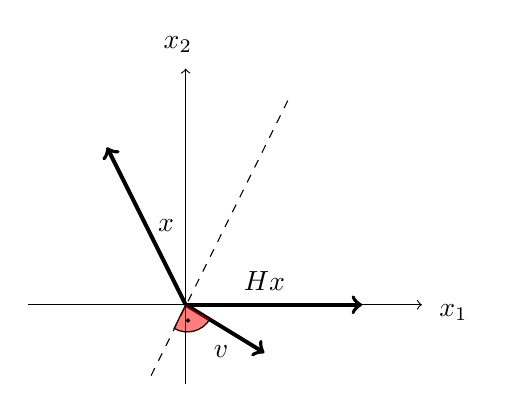
\begin{tikzpicture}

\draw[->] (-2,0) -- (3,0);
\draw[->] (0,-1) -- (0,3);

\draw[->,line width=0.5mm] (0,0) -- (-1,2);
\draw[->,line width=0.5mm] (0,0) -- (2.24,0);

\draw[dashed] (-0.44,-0.9) -- (1.34,2.68);
%\draw[->,line width=0.5mm] (0,0) -- (-0.9, 0.44);
%\draw[->,line width=0.5mm] (0,0) -- (-1,0.61);
\draw[->,line width=0.5mm] (0,0) -- (1,-0.61);





\filldraw[red, opacity=0.5] (0,0)--(-0.1467,-0.3000) arc (240:330:.3339) -- (0,0) ;
\draw[black, opacity=1] (0,0)--(-0.1467,-0.3000) arc (240:330:.3339) -- (0,0) ;
\filldraw(0.03,-0.2) circle (.02cm) ;

%Beschriftung
\draw (3.4,-0.1) node {$x_1$};
\draw (-0.1,3.3) node {$x_2$};

\draw (.45, -.6) node {$v$};
\draw (-.25, 1) node {$x$};
\draw (1,0.3) node {$Hx$};


\end{tikzpicture}}

\end{frame}

\begin{frame}
	\frametitle{Householder-Transformation}
	\vspace{-1cm}
	\begin{itemize}
	\item Householder Vektor berechnen
		\begin{align*}
			Hx = \alpha e_1
		\end{align*}
		$\alpha = -1 \cdot \text{sign}(x_1) \|x\|_2$\\
		$\tau = \dfrac{\alpha - x_1}{\alpha}$\\
		$v=\dfrac{x - \alpha e_1}{x_1 - \alpha}$ 

	\item  Householder-Transformation anwenden
		\begin{align*} 
		H A =(I - \tau vv^T) A= A - \tau (vv^T )A = A - \tau v(v^TA)
		\end{align*}
	\end{itemize}
\end{frame}

\begin{frame}
	\frametitle{QR-Zerlegung mittels Householder}
	\vspace{-4cm}
	\begin{itemize}
		\item $ A = QR $
	\end{itemize}
\end{frame}

\begin{frame}
	\frametitle{Geblockte QR-Zerlegung}
	\begin{itemize}
		\item Matrix A\\
		\centering
		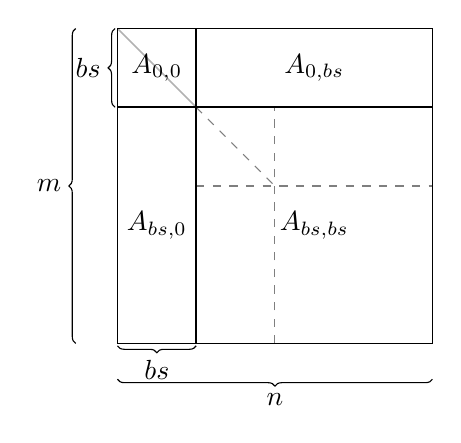
\begin{tikzpicture}
\draw[semithick] (0,0) -- (4,0) -- (4,4) -- (0,4) -- (0,0);

\draw[semithick] (1,0) -- (1,4);
\draw[semithick] (0,3) -- (4,3);
\draw[semithick,opacity=0.3] (0,4) -- (1,3);

\draw[dashed,opacity=0.5] (2,0) -- (2,3);
\draw[dashed,opacity=0.5] (1,2) -- (4,2);
\draw[dashed,opacity=0.5] (1,3) -- (2,2);


\draw (0.5,3.5) node {$A_{0,0}$};
\draw (0.5,1.5) node {$A_{bs,0}$};
\draw (2.5,3.5) node {$A_{0,bs}$};
\draw (2.5,1.5) node {$A_{bs,bs}$};
\draw[decorate, decoration={brace,mirror}, yshift=-.2ex]  (0,0) -- node[below=0.4ex] {$bs$}  (1,0);
\draw[decorate, decoration={brace}, xshift=-.2ex]  (0,3) -- node[left=0.4ex] {$bs$}  (0,4);
\draw[decorate, decoration={brace,mirror}, yshift=-3ex]  (0,0) -- node[below=0.4ex] {$n$}  (4,0);
\draw[decorate, decoration={brace}, xshift=-3.5ex]  (0,0) -- node[left=0.4ex] {$m$}  (0,4);

\end{tikzpicture}
	\end{itemize}
\end{frame}

\begin{frame}
	\frametitle{Householder-Transformationen anwenden}
	\begin{itemize}
		\item Ansatz
		\begin{align*}
			H_1H_2...H_k = I - VTV^T \qquad \text{mit}\qquad H_i = I - \tau_i v_iv_i^T
		\end{align*}
		\item Berechnung vom T
	\end{itemize}
\end{frame}

\begin{frame}
	\frametitle{Householder-Transformationen anwenden}
	\begin{align*}
		C \leftarrow H C = C - V T V^T C \quad %\text{oder} \quad 	%C \leftarrow H^T C = C - V T^T V^T C	\label{eq:larfb}
	\end{align*}
	\centering
	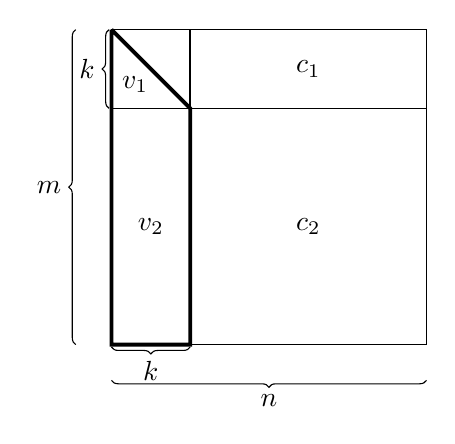
\begin{tikzpicture}
\draw[semithick] (0,0) -- (4,0) -- (4,4)-- (0,4)-- (0,0);


\draw[semithick] (1,0) -- (1,4);
\draw[semithick] (0,3) -- (4,3);
\draw[line width=0.5mm] (0,4) -- (0,0) -- (1,0) -- (1,3) -- (0,4);


\draw[decorate, decoration={brace,mirror}, yshift=-.2ex]  (0,0) -- node[below=0.4ex] {$k$}  (1,0);
\draw[decorate, decoration={brace}, xshift=-.2ex]  (0,3) -- node[left=0.4ex] {$k$}  (0,4);
\draw[decorate, decoration={brace,mirror}, yshift=-3ex]  (0,0) -- node[below=0.4ex] {$n$}  (4,0);
\draw[decorate, decoration={brace}, xshift=-3ex]  (0,0) -- node[left=0.4ex] {$m$}  (0,4);

\draw (0.3,3.3) node {$v_1$};
\draw (0.5,1.5) node {$v_2$};
\draw (2.5,3.5) node {$c_1$};
\draw (2.5,1.5) node {$c_2$};



\end{tikzpicture}

\end{frame}

\begin{frame}
	\frametitle{Ungeblockte QR}
	\centering
	\scalebox{.85}{
		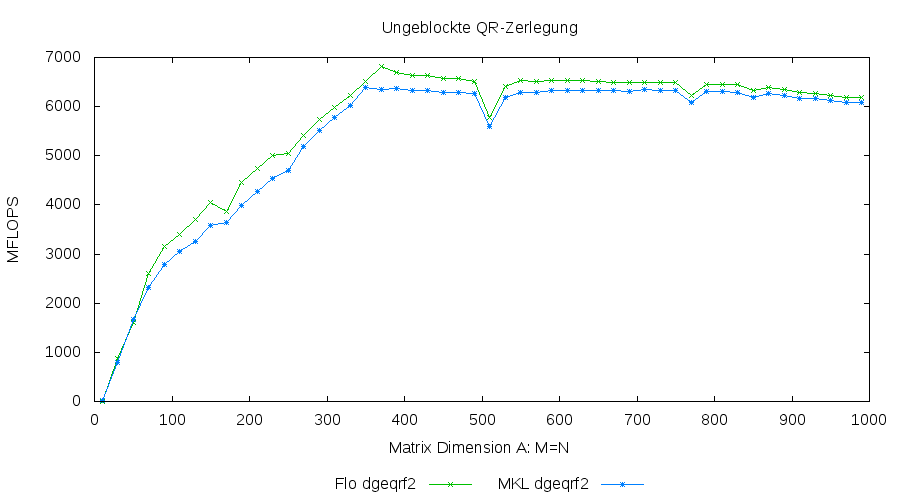
\includegraphics[width=\textwidth]{images/unblk}
	}
\end{frame}

\begin{frame}
	\frametitle{Geblockte QR - Blocksizes}
		\centering
	\scalebox{.85}{
		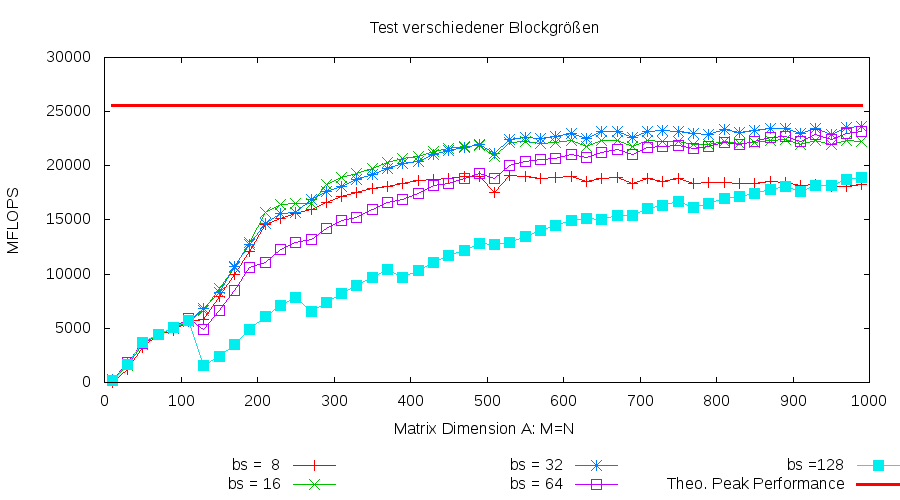
\includegraphics[width=\textwidth]{images/blkbs}
	}
\end{frame}

\begin{frame}
	\frametitle{Geblockte QR}
		\frametitle{Geblockte QR - Blocksizes}
	\centering
	\scalebox{.85}{
		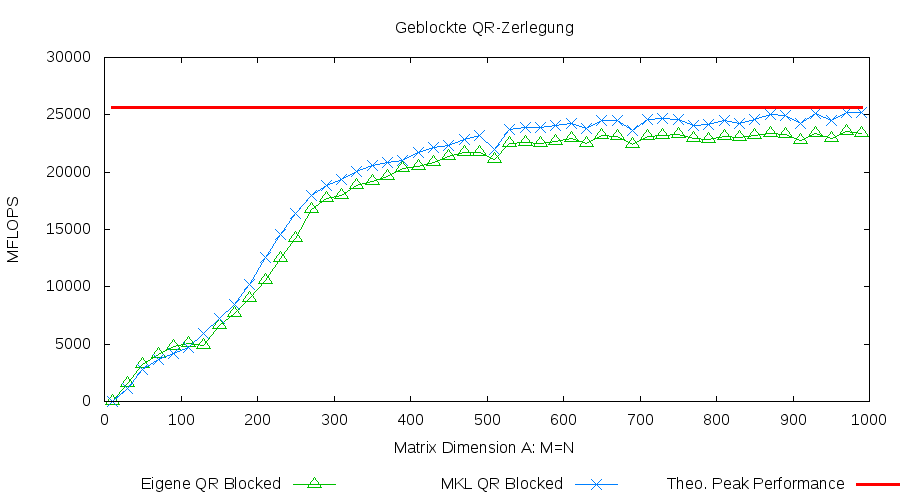
\includegraphics[width=\textwidth]{images/blk}
	}
\end{frame}




